\documentclass{article}
\usepackage[utf8]{inputenc}
\usepackage[hidelinks]{hyperref}
\usepackage[a4paper]{geometry}
\usepackage{amssymb}
\usepackage{graphicx}
\usepackage{fancyhdr}
\usepackage{titlesec}
\usepackage{amsmath}

\titleformat*{\section}{\LARGE\bfseries}
\titleformat*{\subsection}{\Large\bfseries}

\pagestyle{fancy}

\lhead{\leftmark}
\rhead{Page \thepage}
\cfoot{Ojas Karanjkar 210070040}
\renewcommand{\footrulewidth}{1pt}

\begin{document}

\begin{titlepage}
\begin{center}
    \vspace*{\fill}
\includegraphics[scale=0.4]{iitb.png}\\
[4 cm]
    \rule{12.5cm}{0.75mm}\\
    \huge{\bfseries Filter Design Assignment}
    \rule{12.5cm}{0.75mm}\\
    [0.5cm]
   {\textbf {EE338 - 2023 \\
   Elliptic Filter Design Report}}\\
    [2.5cm]
\end{center}
\begin{flushleft}
   {\huge
    Ojas Karanjkar \\
    210070040 \\
     \\}
    \end{flushleft}
\end{titlepage}
\tableofcontents
\thispagestyle{empty}
\clearpage
\pagenumbering{arabic}

\newpage

\section{Student Details}
\begin{itemize}
    \item Name : Ojas Karanjkar
    \item Roll No: 210070040
    \item Filter number assigned: 103
\end{itemize}

\section{Jacobian Elliptic Function}

The elliptic filters are characterised by \textbf{Jacobian Elliptic Function}, which is defined as follows:
The elliptic function \emph{w} = $sn(z, k)$ is defined indirectly through the elliptic integral:\\
\begin{equation}
    z = \int _{0} ^{\phi} \frac{1}{\sqrt{1-k^{2}sin^{2}\theta}} \, d\theta
\end{equation}

Substituting $\emph{w} = sin \phi$ in the above expression,\\
\begin{equation}
    z = \int _{0} ^{\emph{w}} \frac{1}{\sqrt{(1-k^{2}t^{2})(1-t^{2})}} \, dt
\end{equation}

We define following functions based on the Jacobian elliptic functions which will be used in filter design:

\begin{equation}
    \emph{w} = cn(z, k) = cos \phi(z,k)
\end{equation}

\begin{equation}
    \emph{w} = sn(z, k) = sin \phi(z,k)
\end{equation}

\begin{equation}
    \emph{w} = dn(z, k) = \sqrt{1 - k^{2}sn^{2}(z,k)}
\end{equation}

\begin{equation}
    \emph{w} = cd(z, k) = \frac{cn(z,k)}{dn(z,k)}
\end{equation}

Next, we define the complete elliptic integral $K$ which will be used in our filter design:
\begin{equation}
    K = \int _{0} ^{\frac{\pi}{2}} \frac{1}{\sqrt{1-k^{2}sin^{2}\theta}} \, d\theta
\end{equation}

and it's complementary elliptic integral which is defined for k' = $\sqrt{1-k^2}$

\begin{equation}
    K' = \int _{0} ^{\frac{\pi}{2}} \frac{1}{\sqrt{1-k'^{2}sin^{2}\theta}} \, d\theta
\end{equation}

\begin{equation}
    K' = \int _{0} ^{\frac{\pi}{2}} \frac{1}{\sqrt{1-(1-k^{2})sin^{2}\theta}} \, d\theta
\end{equation}

Now that we have defined the functions required for elliptic filter design, we move on to finding the specifications and design our elliptic bandpass and bandstop filters.

\section{Elliptic Bandpass Filter}

\subsection{Un-normailzed Discrete time specifications}

\begin{itemize}
    \item \begin{enumerate}
                \item m = 23
                \item q(m) = [2.3] = 2
                \item r(m) = 23 - 10*2 = 3
                \item BL(m) = 20 + 3*2 + 11*3 = 59
                \item BH(m) = 59 + 75 = 134
            \end{enumerate}

    \item Passband = $59$ kHz to $134$ kHz.
    \item Transition Band Width = $5$ kHz.
    \item Stopband = $0$ to $54$ kHz and $139$ to $300$ kHz.
    \item Tolerance = 0.15.
    \item Nature of Passband = Equiripple.
    \item Nature of Stopband = Equiripple.
\end{itemize}


\subsection{Normailzed discrete filter specifications}
Sampling frequency = $600 kHz$\\
\begin{equation}
    \omega = \frac{\Omega * 2\pi}{\Omega _{sampling}}\\
\end{equation}

\begin{itemize}
    \item Passband = $0.1967\pi$ to $0.4467\pi$ .
    \item Transition Band Width = $0.0167\pi$ .
    \item Stopband = $0$ to $0.18$  and $0.4633\pi$ to $\pi$ .
    \item Tolerance = 0.15.
    \item Nature of Passband = Equiripple.
    \item Nature of Stopband = Equiripple.
\end{itemize}


\subsection{Converting to Analog Low-pass filter}
We have the following transformation for converting into analog low-pass filter:\\
\begin{equation}
    \Omega = tan(\frac{\omega}{2})\\
\end{equation}

Using the above Bilinear Transformation, the passband and stopband specifications are updated as follows:\\

\begin{itemize}
    \item Passband = $0.3191$ to $0.8451$ .
    \item Transition Band = $0.2905$ to $0.3191$ and $0.8451$ to $0.8910$ .
    \item Stopband = $0$ to $0.2905$  and $0.8910$ to $\infty$ .
    \item Tolerance = 0.15.
    \item Nature of Passband = Equiripple.
    \item Nature of Stopband = Equiripple.
\end{itemize}

\subsection{Frequency Transformation for Band-Pass Filter}
The frequency transformation for converting a bandpass filter to low pass filter are as follows:\\

\begin{equation}
    \Omega _{L} = \frac{\Omega^{2} - \Omega_{0}^{2}}{B\Omega}  \\
\end{equation}

\begin{equation}
    B = \Omega _{p2} - \Omega _{p1} \\
\end{equation}

\begin{equation}
    \Omega _{0} = \sqrt{\Omega _{p1}\Omega _{p2}}\\
\end{equation}

According to the above transformation, we can tabulate the updated value of passband and stopband edges:\\

\begin{table}[h]
    \centering
    \begin{tabular}{|c|c|}
        \hline
       $\Omega$ & $\Omega _{L}$\\
       \hline
       $0^+$  & $-\infty$   \\
       \hline
       $0.3191 (\Omega_{p1})$  & $-1$   \\
       \hline
        $0.2905 (\Omega_{s1})$  & $-1.2127$   \\
       \hline
       $0.5193 (\Omega_{0})$  & $0$   \\
       \hline
       $0.8910 (\Omega_{s2})$  & $1.1185$   \\
       \hline
       $0.8451 (\Omega_{p2})$  & $1$   \\
       \hline
       $\infty$  & $\infty$   \\
       \hline
    \end{tabular}
\end{table}

\begin{itemize}
    \item Passband edge = 1 ($\Omega_{lp}$)
    \item Stopband edge = 1.1185 ($\Omega_{ls}$)
    \item Tolerance = 0.15.
    \item Nature of Passband = Equiripple.
    \item Nature of Stopband = Equiripple.
\end{itemize}

\subsection{Parameters for elliptic filter design}
 The general form of a transfer function of a low pass filter is :
 \begin{equation}
     |H(\Omega)|^{2} = \frac{1}{1 + \epsilon _{p}^{2}F_{N}^{2}(\omega)}, \omega = \frac{\Omega}{\Omega_{p}}
 \end{equation}

 In case of elliptic filter, the function $F_{N}(\omega)$ is given by :
 \begin{equation}
     F_{N}(\omega) = cd(NuK_{1}, k_{1}), \omega = cd(uK, k)
 \end{equation}
where,
\begin{equation}
    \epsilon = \sqrt{\frac{2\delta - \delta^{2}}{1-2\delta+\delta^{2}}}
\end{equation}
\begin{equation}
    k_{1} = \frac{\epsilon}{\sqrt{\frac{1}{\delta^{2}}-1}}
\end{equation}
\begin{equation}
    k'_{1} = \sqrt{1-k_{1}^{2}}
\end{equation}
\begin{equation}
    k = \frac{1}{\Omega_{sL}}
\end{equation}
\begin{equation}
    k_{1} = \sqrt{1-k^{2}}
\end{equation}

 The \emph{degree equation} for elliptic filter is:
 \begin{equation}
     N = \frac{KK'_{1}}{K'K_{1}}
 \end{equation}
 To get the minimum order, we take the ceiling of the above mentioned degree equation.\\

We substitute our filter specification in the above mentioned equations to get the parameters for our elliptic bandpass filter.\\

\begin{table}[h]
    \centering
    \begin{tabular}{|c|c|}
    \hline
    parameters & values\\
    \hline
       \epsilon  &  0.6197\\
       \hline
        k & 0.8571\\
        \hline
        K & 2.5508\\
        \hline
        k' & 0.4480\\
        \hline
        K' & 1.1096\\
        \hline
        $k_{1}$ & 0.0940\\
        \hline
        $K_{1}$ & 1.6098\\
        \hline
        $k'_{1}$ & 0.9956\\
        \hline
        $K'_{1}$ & 1.5332\\
        \hline
        N & 3\\
        \hline
    \end{tabular}
\end{table}

\newpage

\subsection{Poles and Zeros}

To find the poles and zeros of the transfer function, we set $N$ = $2L + r$, where $ r \in (0,1)$. Hence for our filter, since N is 3, we get L = 1 and r = 1.\\
Next we define $\zeta _{i}$ = $cd(u_{i}K, k)$ , where $u_{i} = \frac{2i - 1}{N}$ where i = 1,2,.....L\\
Since L = 1, we get $\frac{1}{N} = 0.3333$ and $\zeta = cd(uK,k) = 0.9257$.\\

The zeros of the transfer function is given by \\
\begin{equation}
    z = \frac{j}{k\zeta}
\end{equation}
Plugging in the values, we get $z = 7.9193j$. The other zero is the conjugate of the previously found zero.

For finding the poles of the transfer function, we define 
\begin{equation}
    \nu_{0} = \frac{-j}{NK_{1}}sn^{-1}(\frac{j}{\epsilon},k_{1})
\end{equation}

The expression for polesi is given by :
\begin{equation}
    p = jcd((u-j\nu_{0})K, k)
\end{equation}

If N is odd, we get an additional pole on the real axis, given by \\
\begin{equation}
    p_{0} = jcd((1-j\nu_{0})K, k)
\end{equation}

Finally, we get three poles of given specifications, which are as follows:
$p_{0} = -3.9154$\\
$p_{1} = -0.7246 + j6.2431$\\
$p_{2} = -.07246 - j6.2431$

\subsection{Analog Lowpass Transfer Function}
In the previous section, we found the poles and zeros of our transfer function. From the poles and zeros, we construct the transfer function, which is given by:\\
\begin{equation}
    H_{a}(s) = H_{0}\frac{1}{(1-s/p_{0})} \frac{(1-s/z)(1-s/\Bar{z})}{(1-s/p_{1})(1-s/\Bar{p_{1}})}
\end{equation}

\begin{equation}
    H_{a}(s) = \frac{0.85s^{2} + 53.3077}{s^{3} + 5.3647s^{2} + 45.1753s + 154.6604}
\end{equation}

Next, we apply the transformation \[s_{L} = \frac{\Omega_{0}^2 + s^2}{Bs}\] to get the Bandpass transfer function. 

After applying the transformation, the transfer function for analog bandpass filter becomes:
\begin{equation}
    H_{bpf}(s) = \frac{0.4470s^{5}+7.9958s^{3}+0.0325s}{s^{6}+2.8214s^{5}+13.3044s^{4}+24.0202s^{3}+3.5881s^{2}+0.2052s+0.0196}
\end{equation}

Then we apply the bilinear transformation, to obtain the discrete domain transfer function
\begin{equation}
    H_{bpf}(z) = \frac{0.1885z^{-6}-0.0369z^{-5}-0.4802z^{-4}+0.4802z^{-2}+0.0369z^{-1}-0.1885}{z^{-6}-0.7958z^{-5}-1.3018z^{-4}+0.4283z^{-3}+1.2307z^{-2}-0.3303z^{-1}-0.2032}
\end{equation}

\subsection{Magnitude and Phase response}

\begin{center}
    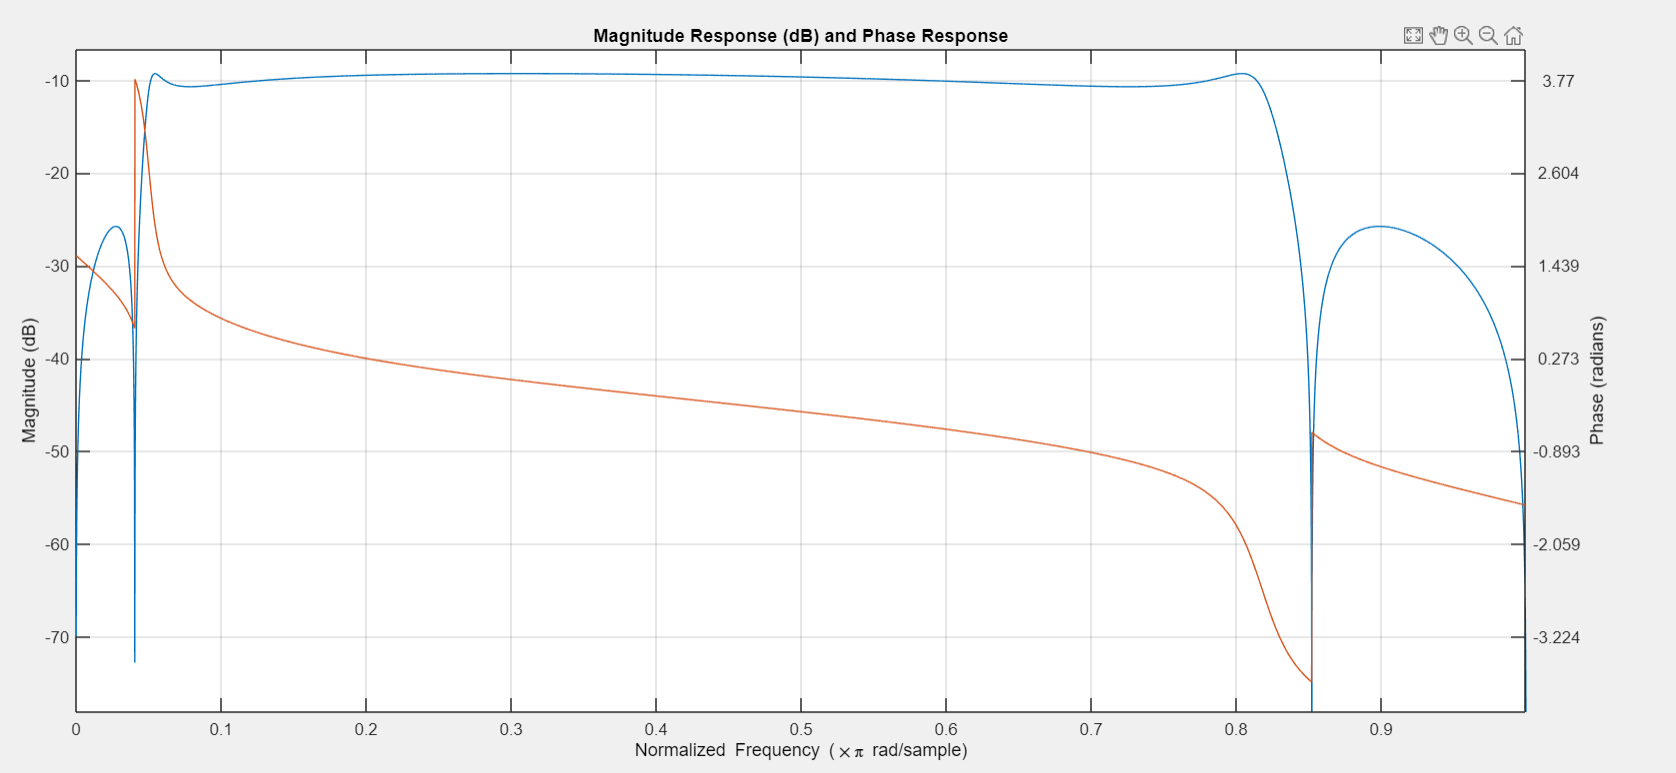
\includegraphics[scale=0.45]{freq_bandpass_ellip.png}\\
    Frequency Response
\end{center}

\begin{center}
    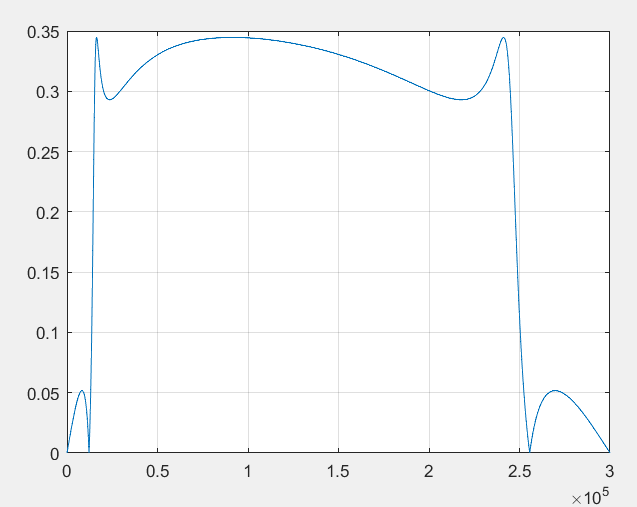
\includegraphics[scale=0.75]{mag_bandpass_ellip.png}\\
    Magnitude plot
\end{center}

\newpage

\section{Elliptic Bandstop Filter}

\subsection{Un-normailzed Discrete time specifications}

\begin{itemize}
    \item \begin{enumerate}
                \item m = 23
                \item q(m) = [2.3] = 2
                \item r(m) = 23 - 10*2 = 3
                \item BL(m) = 20 + 3*2 + 11*3 = 59
                \item BH(m) = 59 + 40 = 99
            \end{enumerate}

    \item Stopband = $59$ kHz to $99$ kHz.
    \item Transition Band Width = $5$ kHz.
    \item Passband = $0$ to $54$ kHz and $104$ to $212.5$ kHz.
    \item Tolerance = 0.15.
    \item Nature of Passband and Stopband : Both equiripple.
\end{itemize}


\subsection{Normailzed discrete filter specifications}
Sampling frequency = $425 kHz$\\
\begin{equation}
    \omega = \frac{\Omega * 2\pi}{\Omega _{sampling}}\\
\end{equation}

\begin{itemize}
    \item Stopband = $0.27\pi$ to $0.46\pi$ .
    \item Transition Band Width = $0.0235\pi$ .
    \item Passband = $0$ to $0.25$  and $0.48\pi$ to $\pi$ .
    \item Tolerance = 0.15.
    \item Nature of Passband and Stopband : Both equiripple.
\end{itemize}


\subsection{Converting to Analog Low-pass filter}
We have the following transformation for converting into analog low-pass filter:\\
\begin{center}
    $\Omega = tan(\frac{\omega}{2})$\\
\end{center}

Using the above Bilinear Transformation, the passband and stopband specifications are updated as follows:\\

\begin{itemize}
    \item Stopband = $0.451$ to $0.88$ .
    \item Transition Band = $0.414$ to $0.4509$ and $0.88$ to $0.939$ .
    \item Passband = $0$ to $0.414$  and $0.939$ to $\infty$ .
    \item Tolerance = 0.15.
    \item Nature of Passband and Stopband : Both equiripple.
\end{itemize}

\subsection{Frequency Transformation for Band-Stop Filter}
The frequency transformation for converting a bandpass filter to low pass filter are as follows:\\

\begin{equation}
    \Omega _{L} = \frac{B\Omega}{\Omega_{0}^{2} - \Omega^{2}}  \\
\end{equation}

\begin{equation}
    B = \Omega _{p2} - \Omega _{p1} \\
\end{equation}

\begin{equation}
    \Omega _{0} = \sqrt{\Omega _{p1}\Omega _{p2}}\\
\end{equation}

According to the above transformation, we can tabulate the updated value of stopband and passband edges:\\

\begin{table}[h]
    \centering
    \begin{tabular}{|c|c|}
        \hline
       $\Omega$ & $\Omega _{L}$\\
       \hline
       $0^+$  & $0^+$   \\
       \hline
       $0.414 (\Omega_{p1})$  & $1.00$   \\
       \hline
        $0.451 (\Omega_{s1})$  & $1.28$   \\
       \hline
       $0.623^- (\Omega_{0})$  & $-\infty$   \\
       \hline
       $0.623^+ (\Omega_{0})$  & $+\infty$   \\
       \hline
       $0.88 (\Omega_{s2})$  & $-1.19$   \\
       \hline
       $0.939 (\Omega_{p2})$  & $-0.99$   \\
       \hline
       $\infty$  & $0^-$   \\
       \hline
    \end{tabular}
\end{table}

\begin{itemize}
    \item Passband edge = 1 ($\Omega_{lp}$)
    \item Stopband edge = 1.19 ($\Omega_{ls}$)
    \item Tolerance = 0.15.
    \item Nature of Passband and Stopband : Both equiripple.
\end{itemize}

\subsection{Parameters for elliptic filter design}
In the previous section on parameters for elliptic bandpass function, I had already discussed the formulae for finding the parameters. Using the same formulae here as well, we get the parameters as follows:

\begin{table}[h]
    \centering
    \begin{tabular}{|c|c|}
    \hline
    parameters & values\\
    \hline
       \epsilon  &  0.6197\\
       \hline
        k & 0.5606\\
        \hline
        K & 2.2898\\
        \hline
        k' & 0.5811\\
        \hline
        K' & 1.1691\\
        \hline
        $k_{1}$ & 0.0940\\
        \hline
        $K_{1}$ & 1.6098\\
        \hline
        $k'_{1}$ & 0.9956\\
        \hline
        $K'_{1}$ & 1.5332\\
        \hline
        N & 2\\
        \hline
    \end{tabular}
\end{table}

\subsection{Poles and Zeros}

For the given specifications for bandstop filter, we get the order to be 2 and hence L = 1 and r = 0.\\
The zeros of the transfer function is given by \\
\begin{equation}
    z = \frac{j}{k\zeta}
\end{equation}
Plugging in the values, we get $z = 15.1550j$. The other zero is the conjugate of the previously found zero.

For finding the poles of the transfer function, we define 
\begin{equation}
    \nu_{0} = \frac{-j}{NK_{1}}sn^{-1}(\frac{j}{\epsilon},k_{1})
\end{equation}

The expression for polesi is given by :
\begin{equation}
    p = jcd((u-j\nu_{0})K, k)
\end{equation}

as N is even, we won't get the additional pole on the X-axis.

Finally, we get two poles of given specifications, which are as follows:
$p_{1} = -2.6696 + j5.7796$\\
$p_{2} = -2.6696 - j5.7796$

\subsection{Analog Lowpass Transfer Function}
In the previous section, we found the poles and zeros of our transfer function. From the poles and zeros, we construct the transfer function, which is given by:\\
\begin{equation}
    H_{a}(s) = \frac{(1-s/z)(1-s/\Bar{z})}{(1-s/p_{1})(1-s/\Bar{p_{1}})}
\end{equation}

\begin{equation}
    H_{a}(s) = \frac{s^{2}+229.6739}{s^{2} + 5.3392s + 40.5307}
\end{equation}

Next, we apply the transformation \[s_{L} = \frac{Bs}{\Omega_{0}^2 + s^2}\] to get the Bandpass transfer function. 

After applying the transformation, the transfer function for analog bandpass filter becomes:
\begin{equation}
    H_{bsf}(s) = \frac{5.6669s^{4}+4.6314s^{2}+0.9433}{s^{4} + 0.0719s^{3} + 0.8234s^{2} + 0.0293s + 0.1665}
\end{equation}

Then we apply the bilinear transformation, to obtain the discrete domain transfer function
\begin{equation}
    H_{bsf}(z) = \frac{5.3761z^{-4}-9.0355z^{-3}+14.5371z^{-2}-9.0355z^{-1}+5.3761}{z^{-4}-1.6352z^{-3}+2.5596z^{-2}-1.5538z^{-1}-0.9032}
\end{equation}

\subsection{Magnitude and Phase response}

\begin{center}
    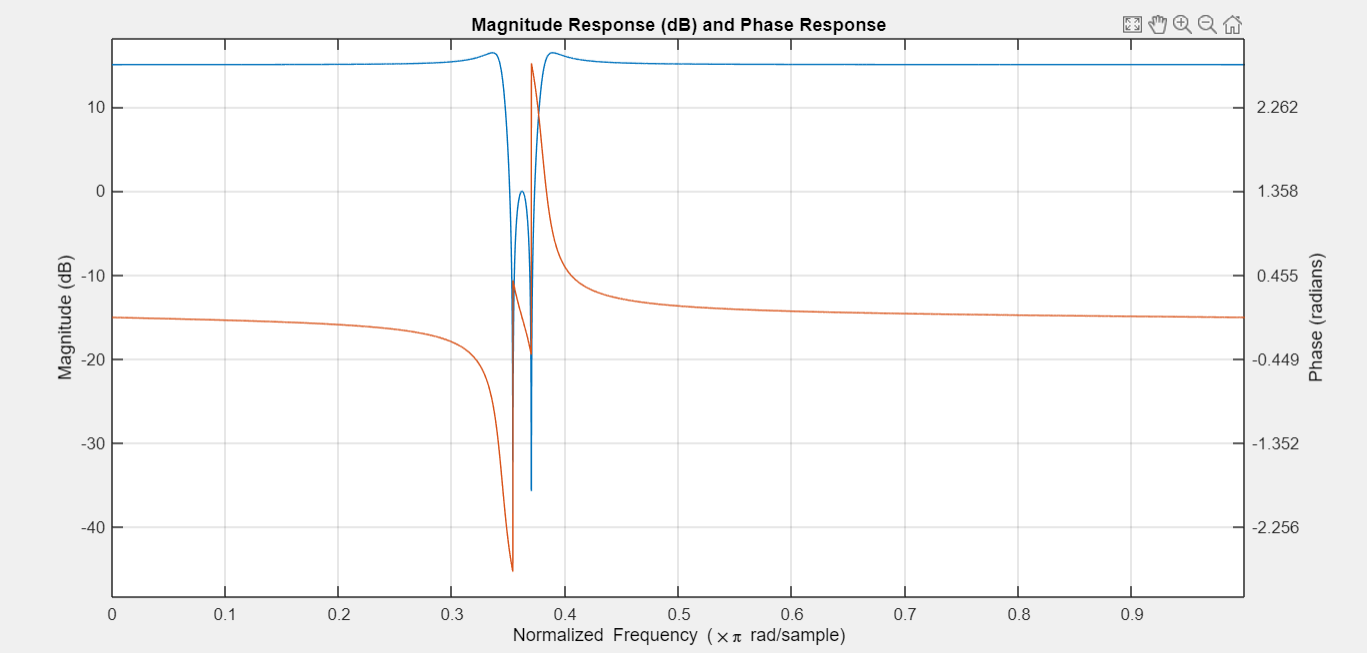
\includegraphics[scale=0.45]{freq_bandstop_ellip.png}\\
    Frequency Response
\end{center}

\begin{center}
    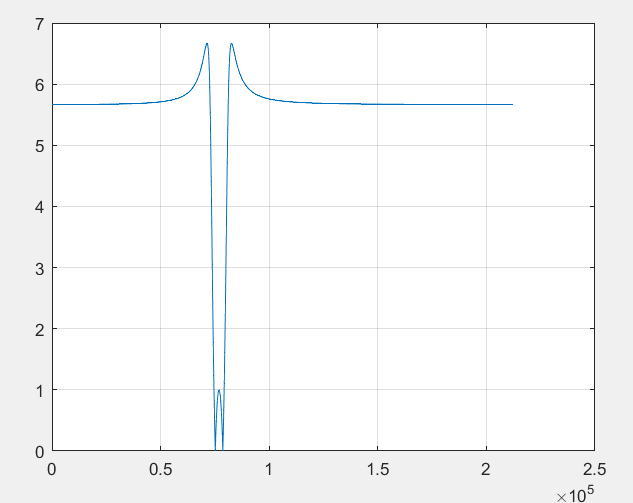
\includegraphics[scale=0.75]{mag_bandstop_ellip.png}\\
    Magnitude plot
\end{center}

\newpage

\section{Comparison between Elliptic and Chebyschev/ Butterworth Filters}

When we compare the order of Elliptic, Chebyschev and Butterworth filter, we observe that the order of Butterworth filter is highest while it is lowest in the case of elliptic filter. However, when we compare the phase response of the three filters, we observe that the phase response of Butterworth filter is most linear among all the three, while it is least linear for Elliptic Filter. Based on the above two observations, we can state that there exist a trade-off between order and the linear phase response. If we try to reduce the order of the filter, the poorer linear phase response we get and vice versa. 



\end{document}
